\chapter[Equivariant cut locus]{Equivariant cut locus}\label{ch:equivariantCutLocusTheorem}
\minitoc

\hfb Let $M$ be a smooth manifold on which a compact Lie group $G$ acts freely. It is known that $M/G$ is a smooth manifold. Moreover, if $M$ has a Riemannian metric and $G$ acts isometrically, then there is an induced Riemannian metric on $M/G$. Let $N$ be a $G$-invariant  submanifold of $M$. We want to find the cut locus of $N/G$ in $M/G$. In this chapter we will discuss the equality between $\cutn/G$ and $\cutn[N/G]$.  We will start the chapter by motivating with an example, then state the theorem and then recall Riemannian submersion which will be useful for the proof of the theorem. At the end we will discuss an application of this result to complex projective hypersurfaces.

\section{Statement of the theorem}
\hfb Let us discuss an example which will be helpful to arrive at the statement of the main theorem. Let $\mathbb{RP}^n$ denotes the $n$-dimensional real projective space which is obtained from $\mathbb{S}^n$ by identifying points $p$ and $-p$. Equivalently, this space can be obtained from the action of $\mathbb{Z}_2$ on $\mathbb{S}^n$. We know from \Cref{eg:CutLocusofPointRPn} that for a point $p\in \mathbb{RP}^n$, the cut locus is $\mathbb{RP}^{n-1}$. In \Cref{join}, we showed that $\mathrm{Cu}\left(\mathbb{S}_i^k\right)=\mathbb{S}_l^{n-k-1}$, where $\mathbb{S}_i^k \hookrightarrow \mathbb{S}^n$ denote the embedding of the $k$-sphere in the first $k+1$ coordinates while $\mathbb{S}^{n-k-1}_l$ denote the embedding of the $(n-k-1)$-sphere in the last $n-k$ coordinates. So we have
\begin{displaymath}
	\begin{tikzcd}
		\mathbb{S}^n \supset\left\{p,-p\right\}\arrow[d,  "\mathbb{Z}_2"] \arrow[rr, "\mathrm{Cu}"] &  &  \mathbb{S}^{n-1} \arrow[d, "\mathbb{Z}_2"]\\
		\mathbb{RP}^n \supset\{p\} \arrow[rr, "\mathrm{Cu}"]& & \mathbb{RP}^{n-1}
	\end{tikzcd}
\end{displaymath}

\noindent Similarly, one can see a similar diagram for the complex projective space $\mathbb{CP}^n$ which is obtained by taking $\mathbb{S}^1$ action on $\mathbb{S}^{{2n+1}}$. We have 
\begin{displaymath}
	\begin{tikzcd}
		\mathbb{S}^{2n+1} \supset \mathbb{S}_i^1 \arrow[d,  "\mathbb{S}^1"] \arrow[rr, "\mathrm{Cu}"] &  &  \mathbb{S}^{2n-1}_f \arrow[d, "\mathbb{S}^1"]\\
		\mathbb{CP}^n \supset\{p\} \arrow[rr, "\mathrm{Cu}"]& & \mathbb{CP}^{n-1}
	\end{tikzcd}
\end{displaymath}

\noindent Thus, it is natural to ask whether the following diagram commutes for a compact Lie group $G$. 
\begin{displaymath}
	\begin{tikzcd}
		M \supset N \arrow[d,  "G"] \arrow[rr, "\mathrm{Cu}"] &  &  \mathrm{Cu}(N) \arrow[d, "G"]\\
		M/G \supset N/G \arrow[rr, "\mathrm{Cu}"]& & \mathrm{Cu}(N)/G
	\end{tikzcd}
\end{displaymath}

\noindent The above diagram make sense if $N$ and $\cutn$ are $G$-invariant subsets. Note that if the action is free and isometric, i.e., length of the curves $\gamma$ and $g\cdot \gamma$ are the same,  then $\mathrm{Se}(N)$ is $G$-invariant. 
\begin{figure}[!htbp]
	\centering
	\begin{subfigure}{.45\textwidth}
		\incfig[0.8]{separatingSetIsG-Invariant-1}
	\end{subfigure}
	\begin{subfigure}{.45\textwidth}
		\incfig[0.8]{separatingSetIsG-Invariant-2}
	\end{subfigure}
	\caption{$\sen$ is $G$-invariant}
\end{figure}
\noindent Now to show that the cut locus of $N$, which is the closure of $\mathrm{Se}(N)$,  is $G$-invariant we take $x\in \overline{\mathrm{Se}(N)}$. So there exists a sequence $\left(x_n\right) \subset \mathrm{Se}(N)$ such that $x_n\to x$ (this convergence is with respect to the Riemannian metric). This implies $g\cdot x_n \to g\cdot x$ as the action is continuous. Hence, $g\cdot x\in \mathrm{Se}(N).$  

\hf The following theorem tells us that the above diagram commutes if $G$ is a compact Lie group and the action is free and isometric.

\begin{thm}[Equivariant cut locus theorem]\label{thm:equivariant-cut-locus}\index{equivariant cut locus theorem}
    Let $M$ be a closed and connected Riemannian manifold  and $G$ be any compact Lie group which acts on $M$ freely and isometrically. Let $N$ be any $G$-invariant closed submanifold of $M$, then we have an equality
    \begin{displaymath}
        \mathrm{Cu}(N)/G = \mathrm{Cu}(N/G).
    \end{displaymath}
\end{thm}

\begin{rem}
	\begin{enumerate}[(i)]
		\item If the action of $G$ is not isometric, then we can construct a $G$-invariant metric on $M$ by averaging any metric on $M$ over $G$. In fact, for any $p\in M$ and any vectors $\mathbf{v}_1,\mathbf{v}_2\in T_pM$, we can define
		\begin{displaymath}
			\left\langle \mathbf{v}_1,\mathbf{v}_2 \right\rangle \defeq \int_G \left\langle \mathbf{v}_1,\mathbf{v}_2 \right\rangle_{g\cdot p}~dg,
		\end{displaymath}
		where the integral is taken with respect to the Haar measure. Then the theorem is valid with respect to the new metric.
		\item Recall that, in \Cref{thm: Morse-Bott}, we proved that the gradient flow of distance squared function from the submanifold $N$ deforms $M-\cutn$ to $N$. By construction, the flow lines are $G$-invariant. So we also have that $M/G-\cutn/G$ deforms to $N/G$.
	\end{enumerate}  
\end{rem}

\vspace{0.3cm}    
\noindent To prove the theorem we have to encounter mainly two problems.
\begin{enumerate}[a.]
	\item Whether a distance minimal geodesic in $M$ projects down to a distance minimal geodesic in $M/G$?
	\item Whether a distance minimal geodesic in $M/G$ lifts to a distance minimal geodesic in $M$?
\end{enumerate}


\section{Proof of the equivariant cut locus theorem} \label{sec:Riemannian-submersion}\index{Riemannian submersion}

\hfb In this section we will recall some results on Riemannian submersion and most of the results can be found in the book \cite[Chapter V, section 26]{Mic08}.

\begin{defn}\label{defn:Ehresmann-connection}
	Let $\pi:E\to B$ be a smooth principal $G$-bundle. An \textit{Ehresmann connection}\index{Ehresmann connection} on $E$ is a smooth subbundle $\mathcal{H}$ of $TE$, called the \textit{horizontal bundle}\index{horizontal bundle} of the connection, such that $TE=\mathcal{H}\directsum \mathcal{V}$, where $\mathcal{V}_p=\ker \left(d\pi_p:T_pE\to T_{\pi(p)}B\right)$.
\end{defn}

\vspace{0.3cm}
\hf The bundle $\mathcal{V}$ is called the \textit{vertical bundle}\index{vertical bundle}, and it is independent of the connection chosen. It follows from the definition that $\mathcal{H}_p$ depends smoothly on $p$ and $\mathcal{H}_p\cap \mathcal{V}_p=\{0\}$. Moreover, the map $d\pi_p$ restricts to $\mathcal{H}_p$ is an isomorphism on $T_{\pi(p)}B$. If $E$ is a Riemannian manifold with metric $g$, then by choosing a horizontal bundle $\mathcal{H}$ we have $\mathcal{H}_p=\mathcal{V}_p^\perp$.

\begin{defn}\label{defn:Riemannian-submersion}
	 A smooth submersion $\pi:(E,g)\to (B,g')$ is called a \textit{Riemannian submersion}\index{Riemannian submersion} if the linear map $d\pi_p$ preserves the length of the horizontal vectors for each point $p\in E$. Equivalently, $d\pi_p$ is a linear isometry between $\mathcal{H}_p$ and $T_{\pi(p)}B$.
\end{defn}

\vspace{0.3cm}
\noindent Using the above definitions we can define the following type of vectors.

\begin{defn}
	Let $\pi:E\to B$ be a Riemannian submersion. A vector field $X\in \mathfrak{X}(E)$ is called
	\begin{itemize}
		\item \textit{vertical} \index{vertical vector field} if for any $p\in E$, $X_p\in \mathcal{V}_p$, denoted by $X^\text{ver}$, and
		\item \textit{horizontal} \index{horizontal vector field} if for any $p\in E$, $X_p\in \mathcal{H}_p$, denoted by $X^\text{hor}$.
	\end{itemize}		
\end{defn}

\vspace{0.3cm}
\noindent We can uniquely decompose any vector field $X\in \mathfrak{X}(E)$ as
\begin{displaymath}
	X = X^\text{ver}+X^{\text{hor}}
\end{displaymath}
into its horizontal and vertical components.

\vspace{0.3cm}
\hf Once we have a connection, we now have a preferred way of lifting vectors from $TB$ to $TE$. Recall that
a vector $\tilde{X}\in T_eE$ is a \textit{lift} of $X\in T_{\pi(e)B}$ if $T_{e}\pi(\tilde{X})=X$. In absence of a connection, there are many different choices of lifts of a vector, and any two choices differ by a vertical vector. That is, if $\tilde{X},\tilde{X}'$ are lifts of $X$,  then $\tilde{X}-\tilde{X}'$ is vertical. Once we have a connection, we can define the \textit{horizontal lift} (with respect to a connection $\mathcal{H}$) of $X$ as the horizontal component of any lift of $X$. This definition
is, of course, independent of the choice of lift, since any two differ by a vertical vector, whose horizontal
component vanishes. Similarly, we can lift vector fields by lifting them in a pointwise fashion.
\begin{defn}[Horizontal lift of vector fields]\index{horizontal lift of a vector field}
	Let $X\in \mathfrak{X}(B)$ be a vector field and $\mathcal{H}\subset TE$ an Ehresmann connection on $E$. We define the \textit{horizontal lift of $X$} as the vector field $\tilde{X}\in \mathfrak{X}(E)$ which satisfies $d\pi(\tilde{X})=X$ and $\tilde{X}_e\in \mathcal{H}_e$ for all $e\in E$.
\end{defn}

\hf Suppose that we have a curve $\gamma:[0,1]\to B$. At each point over the curve, we have a vector $\gamma'(t)\in T_{\gamma(t)}B$, which we can lift to the fiber above $\gamma(t)$. So if we choose a starting point $e_0\in \pi^{-1}(\gamma(0))$, we can find an integral curve along all these lifted vectors on the fibers over the curve $\gamma$. In the end we obtain a curve $\tilde{\gamma}:[0,1]\to E$ satisfying $\pi\circ \tilde{\gamma}=\gamma,~\tilde{\gamma}(0)=e_0$, and $\tilde{\gamma}'(t)\in \mathcal{H}_{\tilde{\gamma}(t)}$ for all $t$. We call it a horizontal lift of $\gamma$.

\begin{defn}[Horizontal lift of a curve]\label{defn:horizontal-lift}\index{horizontal lift of a curve}
	Let $\pi:E\to B$ be a fiber bundle with a connection $\mathcal{H}$. Let $\gamma$ be a smooth curve in $B$ through $\gamma(0)=b$. Let $e\in E$ be such that $\pi(e)=b$. A \textit{horizontal lift}\index{horizontal lift} of $\gamma$ through $e$ is a curve $\tilde{\gamma}$ in $E$ such that $\pi\circ \tilde{\gamma}=\gamma,~\tilde{\gamma}(0)=e$, and $\tilde{\gamma}\kern 0.02cm'(t)\in \mathcal{H}_{\tilde{\gamma}(t)}$.
\end{defn}

\vspace{0.3cm}
\hf For every point $t_0\in (0,1)$, we can find $\epsilon>0$ such that the vector field $\gamma'$ can be extended to a vector field over $\gamma\big|_{(t_0-\epsilon,t_0+\epsilon)}$. Then we look at the horizontal vector field $\tilde{X}$ defined on the bundle $E\big|_{U}$, where $U\supseteq \gamma((t_0-\epsilon,t_0+\epsilon))$. Then $\tilde{\gamma}$ is the integral curve of $\tilde{X}$ starting at the prescribed point $e_0\in \pi^{-1}(\gamma(0))$. Since $[0, 1]$ is compact, a usual gluing argument will help us to construct a horizontal lift of $\gamma$. Hence, we have the following proposition. For a detailed proof of the proposition we refer the reader to \cite[Chapter XIV, Proposition 3.5(i)]{Lang99}.
\begin{prop}\label{prop:uniqueness-of-horizontal-lift}
	Given a smooth path $\gamma:[0,1]\to B$ such that $\gamma(0)=b$ and $e_0\in \pi^{-1}(b)$, there is a unique horizontal lift $\tilde{\gamma}$ of $\gamma$ through $e_0\in E$.
\end{prop}

\vspace{0.3cm}
\noindent Recall the Quotient manifold theorem \cite[Theorem 21.10]{Lee13}.

\begin{thm}[Quotient Manifold Theorem]
	Suppose a Lie group $G$  acting smoothly, freely, and properly on a smooth manifold $M$. Then the orbit space $M/G$ is a topological manifold of dimension equal to $\dim M-\dim G$, and has a unique smooth structure with the property that the quotient map $\pi:M\to M/G$  is a smooth submersion.
\end{thm}

\vspace{0.3cm}
\noindent Using the above theorem, we can define a unique metric on $M/G$ such that $\pi$ is a Riemannian submersion. In fact, for any $x\in M/G$ and $p\in \pi^{-1}(x)$, we take the vertical space $\mathcal{V}_p \defeq \ker d\pi_p$ and the horizontal space $\mathcal{H}_p\defeq \mathcal{V}_p^\perp$ so that $T_pM = \mathcal{V}_p \oplus \mathcal{H}_p$. Since $d\pi_p$ is surjective, then $d\pi_p\big|_{\mathcal{H}_p}:\mathcal{H}_p\to T_{\pi(p)}M/G$ is a bijection. Define 
\begin{displaymath}
	h_x( v,w) \defeq \left\langle d\pi^{-1}\big|_{\mathcal{H}_p}(v),d\pi^{-1}\big|_{\mathcal{H}_p}(w) \right\rangle.
\end{displaymath}
Since the action is isometric, the metric is independent of the choice of point $p$. Thus, $h$ defines a well-defined metric on $M/G$ and $\pi$ is a Riemannian submersion.

\vspace{0.3cm}
\hf The following is the key lemma for proving \Cref{thm:equivariant-cut-locus} and the proof of the same can be found in \cite[Lemma 26.11]{Mic08}.

\begin{lemma}\label{lemma:horizontal-lift-is-a-geodesic}
	Let $\left(E,g_E\right)$ and $\left(B,g_B\right)$ be two Riemannian manifolds and $\pi:E\to B$ be a Riemannian submersion. Let $\gamma$ be a geodesic in $B$ and $\tilde{\gamma}$ be the horizontal lift of $\gamma$. Then we have:
	\begin{enumerate}
		\item The length of $\gamma$ and $\tilde{\gamma}$ are same.
		\item $\tilde{\gamma}'(t)$ is perpendicular to each fiber $E_{\tilde{\gamma}(t)}$.
		\item $\tilde{\gamma}$ is a geodesic in $E$.
	\end{enumerate}
\end{lemma}

\vspace{0.3cm}
\noindent We also have the following result.
\begin{thm}[O'Neill]\label{thm:O'Neill-theorem}
	Let $\pi:E\to B$ be a Riemannian submersion. If $\tilde{\gamma}$ is a geodesic in $E$ and $\tilde{\gamma}'(0)\in \mathcal{H}_{\tilde{\gamma}(0)}$, then $\tilde{\gamma}'(t)\in \mathcal{H}_{\tilde{\gamma}(t)}$ for all $t$. Moreover, $\pi\circ \tilde{\gamma}$ is a geodesic in $B$ and the length is preserved.
\end{thm}

\vspace{0.3cm}
\noindent The above theorem can also be proved using \Cref{lemma:horizontal-lift-is-a-geodesic}, see \cite[Corollary 26.12]{Mic08}.

\vspace{.3cm}

\noindent Combining \Cref{lemma:horizontal-lift-is-a-geodesic} and \Cref{thm:O'Neill-theorem}, we have the following correspondence. 

\begin{thm}\label{thm:geodesic-correspondence}
	There is a one-to-one correspondence between the geodesics on $M/G$ and geodesics on $M$ which are horizontal.
\end{thm}

\vspace{.3cm}
\noindent We now ready to prove \Cref{thm:equivariant-cut-locus}.

\begin{proof}[Proof of \Cref{thm:equivariant-cut-locus}]
	Note that if $\tilde{\gamma}$ is an $N$-geodesic, then $\tilde{\gamma}'(1)\in \mathcal{H}_{\tilde{\gamma}(1)}$ and from \Cref{thm:O'Neill-theorem} $\tilde{\gamma}'(t)\in \mathcal{H}_{\tilde{\gamma}(t)}$ and hence $\tilde{\gamma}$ is a horizontal geodesic which implies $\gamma=\pi\circ \tilde{\gamma}$ is a geodesic in $M/G$.

	\hf Let $\tilde{p}\in \mathrm{Se}(N)$. This implies there exists at least two $N$-geodesic, say $\tilde{\gamma}$ and $\tilde{\eta}$ such that $l(\tilde{\gamma})=l(\tilde{\eta})=d(\tilde{p},N)$. Let us denote $\gamma=\pi\circ \tilde{\gamma}$ and $\eta = \pi\circ\tilde{\eta}$. Due to uniqueness of horizontal lift (\Cref{prop:uniqueness-of-horizontal-lift}), $\gamma$ and $\eta$ will be two different geodesics and the lengths will be same. Also, note that as $\tilde{\gamma}$ is an $N$-geodesic, $\gamma$ will be an $N/G$ geodesic. Otherwise, there exists an $N/G$-geodesic $\delta$ joining $p$ to $N/G$ which gives a horizontal lift $\tilde{\delta}$ whose length is strictly less than $\tilde{\gamma}$, a contradiction (see \Cref{fig:Se(N)/G-subset-Se(N/G)}). Hence, $\pi(\tilde{p})\in \mathrm{Se} (N/G)$. 
	\begin{figure}[!htb]
		\centering
		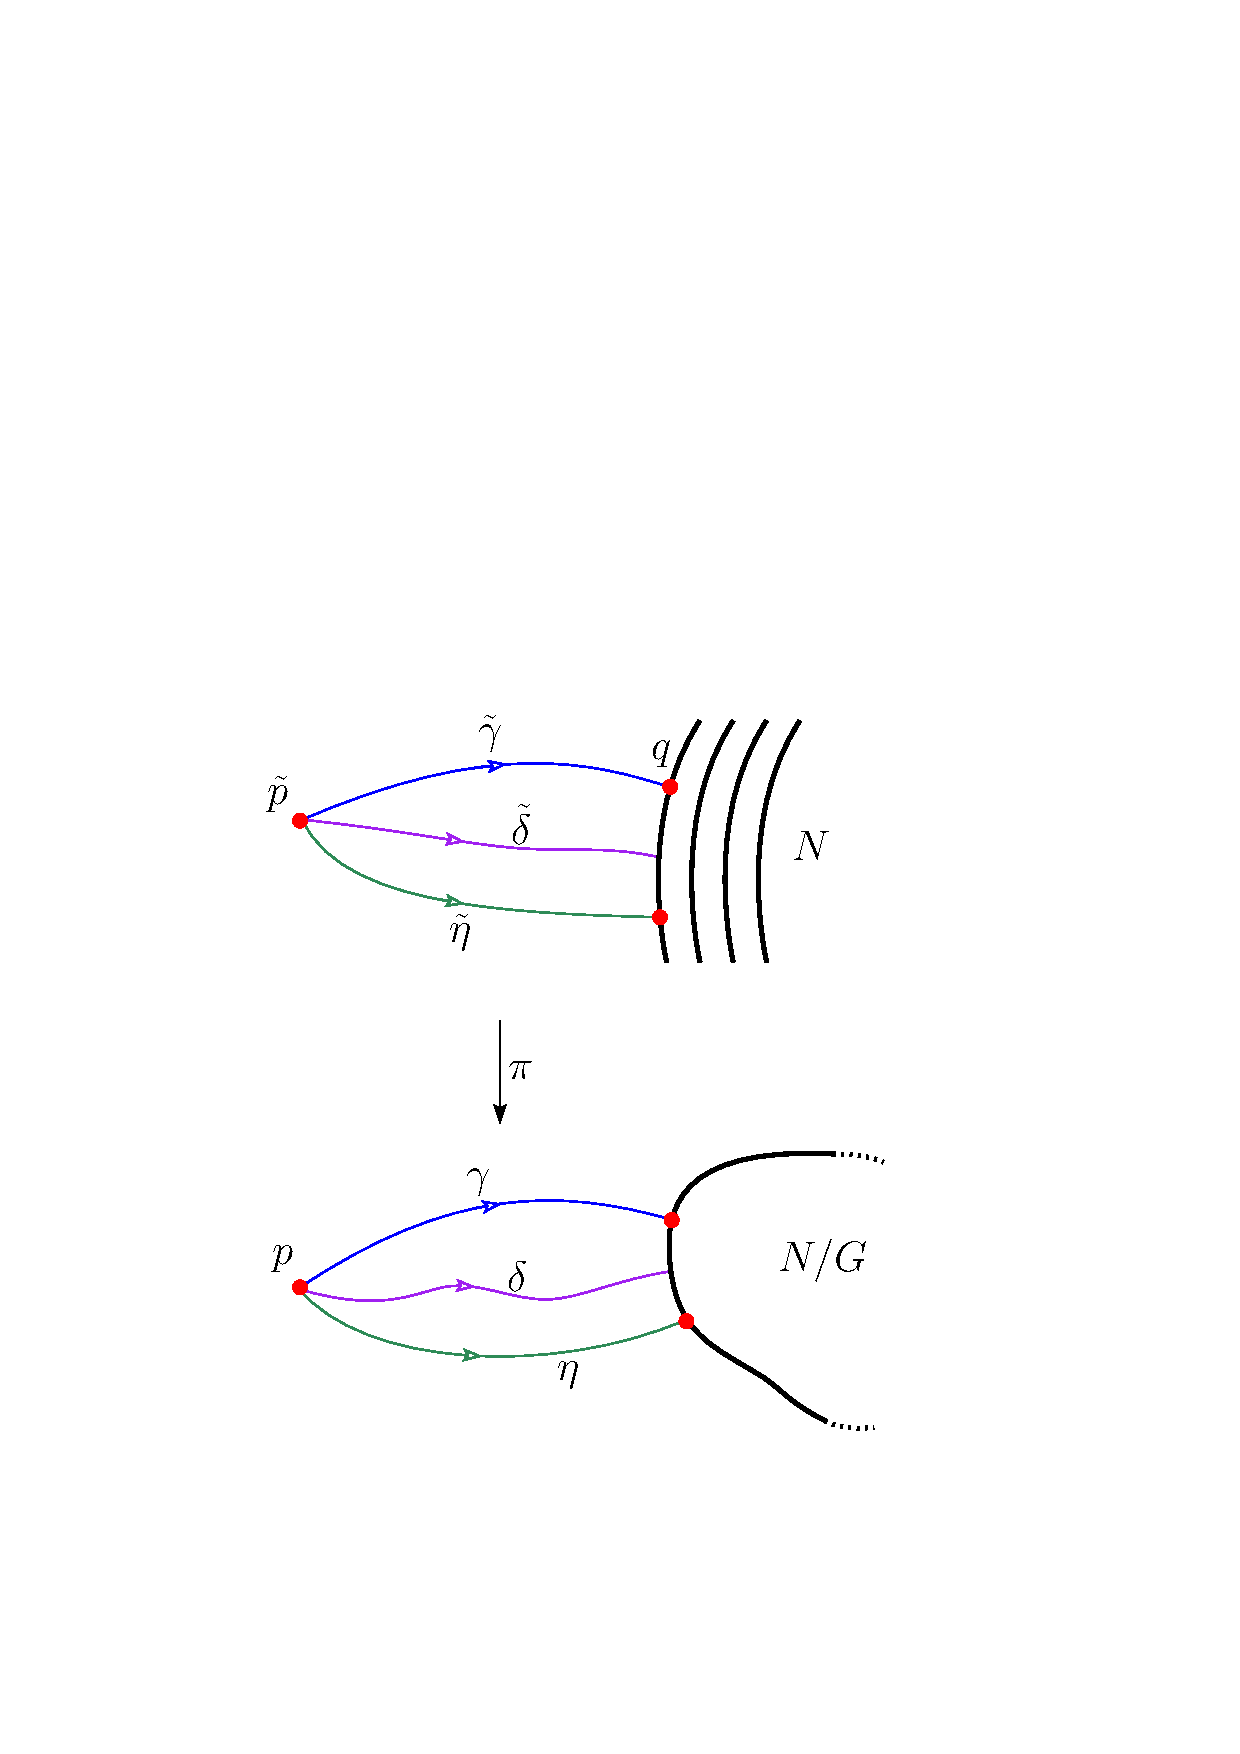
\includegraphics[width=0.5\textwidth]{figures/proof_of_the_main_theorem-one-side.pdf}
		\caption{$N$-geodesics maps to $N/G$-geodesics}
		\label{fig:Se(N)/G-subset-Se(N/G)}
	\end{figure}
	On the other hand, if $\gamma$ is an $N/G$ geodesic starting from $p$, then its horizontal lift $\tilde{\gamma}$ will be a geodesic. In fact, it will be an $N$-geodesic. If not, let $\tilde{\eta}$ be such that $l \left(\tilde{\eta}\right)=d \left(\tilde{p},N\right)$ which implies $\tilde{\eta}$ is horizontal. Hence, $\eta$ will be a geodesic and 
	\begin{align*}
		l(\gamma) & =  d \left(p,N/G\right) = l(\eta) \\ 
		& = l \left(\tilde{\eta}\right) < l \left(\tilde{\gamma}\right) = l(\gamma),
	\end{align*}
	a contradiction. 
	Thus $\tilde{p}\in \mathrm{Se}(N)$. This proves that $\mathrm{Se}(N)/G=\mathrm{Se}(N/G)$. In order to prove the theorem, note that we have the following relation. 
	\begin{displaymath}
		\mathrm{Se}(N/G) \subseteq \overline{\sen}/G \subseteq \overline{\mathrm{Se}(N/G)}.
	\end{displaymath}
	As $\overline{\sen}$ is a closed set and $G$ is a compact Lie group, so $\overline{\sen}/G$ is closed. Thus, we have 
	\begin{displaymath}
		\overline{\sen}/G = \overline{\mathrm{Se}(N/G)} \implies \cutn/G=\cutn[N/G].
	\end{displaymath}
\end{proof}

\hf We will discuss some examples based on the above result. Recall from \Cref{join}, 
\begin{displaymath}
	 \mathrm{Cu} \left(\sbb^k_i\right)=\sbb^{n-k-1}_l.
\end{displaymath}
\begin{eg}[Real projective spaces]
	Take $M=\sbb^{n},~N=\sbb^{k}_i$ and $G=\sbb^0\cong \mathbb{Z}_2$. Applying \Cref{thm:equivariant-cut-locus}, we get
	\begin{displaymath}
		\mathrm{Cu}\left(\mathbb{RP}^k_i\right) \cong \mathbb{RP}^{n-k-1}_l.
	\end{displaymath}
\end{eg}

\begin{eg}
	Take $M=\sbb^{2n+1},~N=\sbb^{2k+1}_i$ and $G=\sbb^1$. Applying \Cref{thm:equivariant-cut-locus}, we get
	\begin{displaymath}
		\mathrm{Cu}\left(\mathbb{CP}^k_i\right) \cong \mathbb{CP}^{n-k-1}_l.
	\end{displaymath}
\end{eg}

\begin{eg}[Lens space]
	Consider $\sbb^{2n+1}\subset \cbb^{n+1}$. Let $p$ be a prime number and $\xi=e^{\frac{2\iota\pi}{p}}$ be a primitive $p^{\text{th}}$ root of unity and let $q_1,\cdots,q_{n+1}$ be integers coprime to $p$. Consider $\zbb_p=\left\{1,\xi,\xi^2,\cdots, \xi^{p-1}\right\}$ and let it acts on $\sbb^{2n+1}$ by $\xi \left(z_1,\cdots,z_{n+1}\right)\defeq \left(\xi^{q_1}z_1,\cdots,\xi^{q_{n+1}}z_{n+1}\right)$. The orbit space is denoted by $L(p;q_1,\ldots,q_{n+1})$ and is called a \emph{lens space}.\index{lens spaces} Since $\mathrm{Cu} \left(\sbb^{2n-1}\subset \sbb^{2n+1}\right)=\sbb^1$, so taking the $\zbb_p$ action, gives that the cut locus of $L\left(p;q_1,\ldots,q_n\right)$ in $L \left(p;q_1,\ldots,q_{n+1}\right)$ is $\sbb^1$. In general, we have
	\begin{displaymath}
		\mathrm{Cu}\left(L \left(p;q_1,\ldots,q_{k+1}\right)\right) \cong L \left(p;q_{k+2},\ldots,q_{n+1}\right).
	\end{displaymath}
\end{eg}


\section{Cut locus of hypersurface in complex projective space}\label{subsec:cut-locus-for-X(d)} 

\hfb Let $\zbf=\left(z_0,\cdots,z_{n}\right)\in \mathbb{C}^{n+1}$ and $[\zbf]\in \mathbb{CP}^{n}$, then the Fermat hypersurface of degree $d$ is given by the polynomial $f(\zbf) = z_0^d+\cdots+z_{n}^d$, 
\begin{displaymath}
	X(d) \defeq \{[\zbf]:f(\zbf)=0\}.
\end{displaymath} 

\noindent The homotopy type of the complement of the above hypersurface is well studied in the article \cite{KuWo80}. Since the partial derivatives $\frac{\partial f}{\partial z_j}$ do not vanish simultaneously on $\mathbb{C}^{n+1}-\{0\}$, the hypersurface is nonsingular. We wish to find its cut locus and want to compare our result with the result in \cite[Proposition 3.1]{KuWo80}. In that paper, the authors found the homotopy type of the complement of the hypersurface.
\begin{prop}[\cite{KuWo80}]
	The complement of $X(d)$ is homotopic to the base space of the $n$ universal principal $\mathbb{Z}_d$-bundle constructed by Milnor from the join of $n+1$ copies of $\mathbb{Z}_d$.  
\end{prop}

\vspace{0.3cm}
\noindent Using \Cref{thm: Morse-Bott}, the same can be studied by looking at the cut locus of $X(d)$ in $\mathbb{CP}^n$. We will use \Cref{thm:equivariant-cut-locus} to find the cut locus of $X(d)$. Recall that there is a principal $\mathbb{S}^1$-bundle given by
\begin{displaymath}
	\pi:\mathbb{S}^{2n+1}\to \mathbb{CP}^n,~ (z_0,\cdots,z_n)\mapsto [z_0:\cdots:z_n].
\end{displaymath} 
Therefore, using \Cref{thm:equivariant-cut-locus} it is enough to find the cut locus of $\pi^{-1}(X(d))\defeq \tilde{X}(d)$. We propose the following conjecture.

\begin{conj}\label{conj:cut-locus-of_X(d)}
	The cut locus of $\tilde{X}(d)\subseteq \sbb^{2n+1}$ is $\zbb_d^{\star(n+1)}\times_{\zbb_d}\sbb^1$, where $\times_{\mathbb{Z}_d}$ is the diagonal action of $\mathbb{Z}_d$ and $\star$ denotes the topological join of spaces.  
\end{conj}

\vspace{0.3cm}
\noindent Using \Cref{thm:equivariant-cut-locus}, the cut locus of $X(d)$ will be $\mathbb{Z}_d^{\star(n+1)}$ and hence we are recovering the $n^{\text{th}}$-stage of Milnor join construction of classifying space for $\mathbb{Z}_d$. Note that we can see $\zbb_d\subset \sbb^1$ and $\mathbb{S}^{2n+1}$ is the join of $n$ circles. Hence, $\zbb_d^{\star(n+1)}\subset \sbb^{2n+1}$ and also note that 
\begin{displaymath}
	 \zbb_d^{\star(n+1)} \times \mathbb{S}^1 \hookrightarrow \sbb^{2n+1},~ \left(\vbf,e^{\iota\theta}\right) \mapsto \vbf e^{-\iota\theta}
\end{displaymath}
gives a well-defined map from $\zbb_d^{\star(n+1)} \times_{\zbb_d}\sbb^1$ to $\sbb^{2n+1}$. We will prove some particular cases of the above conjecture. More precisely, we will prove the above conjecture holds for $d=2$ and arbitrary $n$ (\Cref{thm:cut-locus-of_Xn_2}) and $n=1$ and  arbitrary $d$ (\Cref{thm:cut-locus-for_X1_d}). Let us denote 
\begin{displaymath}
	\widetilde{\mathrm{Cu}}= \mathrm{Cu} (\tilde{X}(d)),\text{ and } \widetilde{\mathrm{Se}}= \mathrm{Se} (\tilde{X}(d)).
\end{displaymath}

\begin{thm}[Cut locus of $X(2)$] \label{thm:cut-locus-of_Xn_2}
	The cut locus of $\tilde{X}(2)\subseteq \sbb^{2n+1}$ is $\sbb^{n}\times_{\zbb_2}\sbb^1\cong \{(\vbf\cos \theta,\vbf\sin\theta):\vbf\in \sbb^n,\theta\in [0,2\pi]\}$. Hence, the cut locus of $X(2)$ in $\CP^{n}$ will be $\mathbb{RP}^{n+1}$.
\end{thm}

\begin{proof}
	We will show that $\{(\vbf\cos \theta,\vbf \sin\theta):\vbf\in \sbb^n,\theta\in \rbb\} = \mathrm{Se}(\tilde{X}(2))$. Let $\vbf\in \sbb^n$ and $\theta\in \rbb$. Let us write $z_j=x_j+\iota y_j$. We can write $\tilde{X}(2)$ as
	\begin{align*}
		\tilde{X}(2) & = \left\{\left(z_0,\cdots,z_n\right)\in \cbb^{n+1}:\sum_{i=0}^n z_i^2=0,\text{ and } \sum_{i=0}^n\left|z_i\right|^2=1\right\} \\ 
		& = \left\{ \left(x_0,y_0,\cdots,x_n,y_n\right): \sum_{i=0}^nx_i^2=\frac{1}{2}=\sum_{i=0}^{n} y_i^2,\text{ and } \sum_{i=0}^{n} x_iy_i=0	\right\} \\
		& = \left\{ \left(x_0,x_1,\cdots,x_n,y_0,y_1,\cdots,y_n\right): \sum_{i=0}^nx_i^2=\frac{1}{2}=\sum_{i=0}^{n} y_i^2,\text{ and } \sum_{i=0}^{n} x_iy_i=0	\right\}.
	\end{align*}
	If $A\in O(n+1)$, then $\tilde{A}=\left(\begin{array}[]{c|c}
		A & \mathbf{0}   \\ \hline 
		\mathbf{0}  & A
	\end{array}\right)\in SO(2n+2)$. Note that
	\begin{enumerate}
		\item[i] $\tilde{A}\in \mathrm{Iso}\left(\sbb^{2n+1}\right)$, where $\mathrm{Iso}(M)$ denotes the set of all isometries of $M$. 
		\item[ii] $\tilde{A}$ maps $\tilde{X}(2)$  to itself, and $\widetilde{\mathrm{Cu}}$ to itself. 
	\end{enumerate}
	Thus, if $p\in \widetilde{\mathrm{Se}}\subseteq \widetilde{\mathrm{Cu}}$ and let $\gamma$ and $\eta$ be two distance minimal geodesics joining $p$ to $\tilde{X}(2)$, then $\tilde{A}\gamma$ and $\tilde{A}\eta$ will be two minimal geodesics joining $\tilde{A}p$ to $\tilde{X}(2)$. As the action of $O(n+1)$ on $\sbb^n$ is transitive, it suffices to check if $\ebf _1\cos\theta+\ebf_{n+2}\sin \theta\in \widetilde{\mathrm{Se}}$. We can further reduce our work by looking at the matrix 
	\begin{displaymath}
		B = 
		\begin{pmatrix}
			\begin{array}{cccc|cccc}
				\cos \theta  & 0 & \cdots & 0 & \sin \theta & 0 & \cdots & 0 
				\\
				0 &  &&   & 0 &  && 
				\\
				\vdots &  &I_n&   & \vdots &  &\bigzero_n& 
				\\
				0 &  &&   & 0 &  &&  
				\\ \hline
				-\sin \theta  & 0 & \cdots & 0 & \cos \theta & 0 & \cdots & 0 
				\\
				0 &  &&   & 0 &  && 
				\\
				\vdots &  &\bigzero_n&   & \vdots &  &I_n& 
				\\
				0 &  &&   & 0 &  &&  
				\\
			\end{array}
		\end{pmatrix},
	\end{displaymath}
	which is again an isometry of $\sbb^{2n+1}$ and sends $\ebf _1\cos\theta+\ebf_{n+2}\sin \theta$ to $\ebf_1$. Hence, it is enough to prove that $\ebf _1\in \widetilde{\mathrm{Se}}$.
	Note that 
	\begin{displaymath}
		\dist \left(\ebf_1,\tilde{X}(2)\right)=\frac{\pi}{4}.
	\end{displaymath}
	Let
	\begin{displaymath}
		 \vbf_1 = \ebf_{2n+2},~\vbf_2=-\ebf_{2n+2}.
	\end{displaymath}
	Consider the geodesics 
	\begin{displaymath}
		 \gamma(t)=\ebf_1\cos t+\ebf_{2n+2}\sin t,\text{ and } \eta(t) = \ebf_1\cos t-\ebf_{2n+2}\sin t,~t\in \mathbb{R}. 
	\end{displaymath}
	Note that $\gamma$ and $\eta$ intersect the set $\tilde{X(2)}$ at $t=\frac{\pi}{4}$, so their lengths are same, and it is equal to the distance between $\ebf_1$ and the submanifold. This proves that $\ebf_1\in \widetilde{\mathrm{Se}}$. 

	\hf Conversely, if $p = (\vbf,\wbf)\in \widetilde{\mathrm{Se}}$, then we will show that there exists $\ubf \in \sbb^n$ and $\theta\in \rbb$ such that $\vbf = \ubf \cos \theta$ and $\wbf=\ubf\sin \theta$. Note that if $\{\vbf,\wbf\}$ is linearly dependent, then there exists $\theta\in \rbb$ such that 
	\begin{displaymath}
		 \vbf = \hat{\vbf}\cos \theta,~~ \wbf = \hat{\vbf}\sin \theta
	\end{displaymath}
	and hence $p\in \widetilde{\mathrm{Se}}$. So we assume that $\vbf$ and $\wbf$ are linearly independent. Suppose $p\notin \sbb^n\times_{\zbb_2} \sbb^1$. We need to show that $p\notin \widetilde{\mathrm{Se}}$. To the contrary, let us assume that $p\in \widetilde{\mathrm{Se}}$. Consider a unit speed geodesic $\gamma(t)$ in the direction of $\vbb=(\vbf_1,\vbf_2)\in T_{(\vbf,\wbf)}\sbb^{2n+1}$ which implies 
	\begin{align}
		\left\|\vbf_1\right\|^2+\left\|\vbf_2\right\|^2=1 \label{eq:tangent_space_of_sphere_cond-1} \\ 
		\left\langle \vbf_1, \vbf \right\rangle + \left\langle \vbf_2, \wbf \right\rangle=0 \label{eq:tangent_space_of_sphere_cond-2}
	\end{align}
	Consider the curve $\gamma(t)=\left(\vbf\cos t+\vbf_1\sin t, \wbf\cos t+\vbf_2\sin t\right)$ for $t\in \mathbb{R}$. Note that $2\le \operatorname{rank}[\vbf,\wbf,\vbf_1,\vbf_2] \le 4$. We will prove that none of the cases is possible. Since $p\in \widetilde{\mathrm{Se}}$, so $p\in \widetilde{\mathrm{Cu}}$ which implies there exists $t\in \rbb$ such that $\gamma(t)\in \tilde{X}(2),\gamma'(t)\in \left(T_{\gamma(t)}\tilde{X}(2)\right)^\perp$ and $t$ will be minimum among all such values. So we have
	\begin{align}
		& \left\|\vbf\right\|^2\cos^2t+\left\|\vbf_1\right\|^2\sin^2t+\left\langle \vbf, \vbf_1 \right\rangle \sin 2t = \frac{1}{2} \label{eq:geodesic-on-X(2)-1},
		\\
		& \left\|\wbf\right\|^2\cos^2t+\left\|\vbf_2\right\|^2\sin^2t+\left\langle \wbf, \vbf_2 \right\rangle \sin 2t = \frac{1}{2}, \notag
		\\
		& \left\langle \vbf, \wbf \right\rangle\cos^2t + \left\langle \vbf_1, \vbf_2 \right\rangle\sin^2t + \frac{1}{2} \left(\left\langle \vbf, \vbf_2 \right\rangle + \left\langle \vbf_1, \wbf \right\rangle\right)\sin 2t=0\label{eq:geodesic-on-X(2)-3}. 
	\end{align}
	Now we will make use of the other condition $\gamma'(t)\in \left(T_{\gamma(t)}\tilde{X}(2)\right)^\perp$. Consider the vector $\ubb= \left(-\wbf\cos t+\vbf_2\sin t,\vbf\cos t+\vbf_1\sin t\right)$. We claim that $\ubb\in T_{\gamma(t)}\tilde{X}(2)$. Note that $(\vbf,\wbf)\in T_{(\mathbf{p},\mathbf{q})}\tilde{X}(2)$ implies $\left\langle \mathbf{p} ,\vbf  \right\rangle=0, \left\langle \mathbf{q} ,\wbf  \right\rangle=0$ and $\left\langle \mathbf{p} ,\wbf  \right\rangle+ \left\langle \mathbf{q} , \vbf  \right\rangle=0$. 
	\begin{align*}
		\left\langle \mathbf{p}, \vbf \right\rangle & = \left\langle \left(\vbf \cos t+\vbf_1\sin t\right), \left(-\wbf \cos t-\vbf_2\sin t\right) \right\rangle 
		\\
		& = - \left\langle \vbf, \wbf \right\rangle\cos^2t-\left\langle \left(\vbf,\vbf_2 \right\rangle + \left\langle \vbf_1, \wbf \right\rangle \right) \cos t \sin t - \left\langle \vbf_1, \vbf_2 \right\rangle\sin^2t 
		\\
		& = 0 \qquad (\text{from \eqref{eq:geodesic-on-X(2)-3}}).
	\end{align*}
	Similarly, $\left\langle \mathbf{q}, \wbf \right\rangle=0$, and 
	\begin{align*}
		& \kern 0.5cm \left\langle \mathbf{p}, \wbf \right\rangle + \left\langle \mathbf{q}, \vbf \right\rangle \\
        & = \left\langle \vbf \cos t+\vbf_1\sin t, \vbf\cos t+\vbf_1\sin t  \right\rangle + \left\langle \wbf\cos t+\vbf_2\sin t, -\wbf\cos t-\vbf_2\sin t \right\rangle 
		\\
		& = \left\|\vbf\right\|^2\cos^2t + \left\|\vbf_1\right\|^2\sin^2t + 2 \left\langle \vbf,\vbf_1\right\rangle\cos t\sin t - \left\|\wbf\right\|^2\cos^2t-\left\|\vbf_2\right\|^2\sin^2t 
		\\ 
		& \kern 2cm - 2 \left\langle \wbf, \vbf_2 \right\rangle\cos t \sin t  
		\\ 
		& = \cos^2t \left(\left\|\vbf\right\|^2-\left\|\wbf\right\|^2\right)+ \sin^2t \left(\left\|\vbf_1\right\|^2-\left\|\vbf_2\right\|^2\right) + \sin 2t \left(\left\langle \vbf,\vbf_1 \right\rangle - \left\langle \wbf,\vbf_2 \right\rangle\right) 
		\\ 
		& = 0 \qquad (\text{from \eqref{eq:tangent_space_of_sphere_cond-1} and \eqref{eq:tangent_space_of_sphere_cond-2}}). 
	\end{align*}
	Therefore, $\ubb\in T_{\gamma(t)}\tilde{X}(2)$ and hence $\left\langle \ubb, \gamma'(t) \right\rangle = 0$ which implies 
	\begin{equation}
		\left\langle \vbf,\vbf_2 \right\rangle - \left\langle \vbf_1,\wbf \right\rangle = 0 \label{eq:perp-cond}.
	\end{equation}
	Define 
	\begin{displaymath}
		\tilde{\ubf}_1 = \sqrt{2} \left(\vbf\cos t+\vbf_1\sin t\right),\text{ and } \tilde{\ubf}_2 = \sqrt{2} \left(\wbf\cos t+\vbf_2\sin t\right).
	\end{displaymath}
	Note that $\tilde{\ubf}_1\perp \tilde{\ubf}_2$ and both are vectors in $\rbb^{n+1}$. We extend $\left\{\tilde{\ubf}_1,\tilde{\ubf}_2\right\}$ to an orthonormal basis of $\rbb^{n+1}$, say $\left\{\tilde{\ubf}_1,\tilde{\ubf}_2, \tilde{\ubf}_3,\ldots,\tilde{\ubf}_{n+1}\right\}$. If $\left(\wbf_1,\wbf_2\right)\in T_{\gamma(t)}\tilde{X}(2)$, then $\left\langle \wbf_1,\tilde{\ubf}_1 \right\rangle=0$, $\left\langle \wbf_2,\tilde{\ubf}_2 \right\rangle=0$ and $\left\langle \wbf_1,\tilde{\ubf}_2 \right\rangle+\left\langle \wbf_2,\tilde{\ubf}_1 \right\rangle=0$ as $\gamma(t) = \frac{1}{\sqrt{2}}(\tilde{\ubf}_1,\tilde{\ubf}_2)$. This implies $\wbf_1,\wbf_2\in \operatorname{Span}\left\{\tilde{\ubf}_3,\ldots,\tilde{\ubf}_{n+1}\right\}$ or 
	\begin{displaymath}
		 \wbf_1=-\tilde{\ubf}_2+\sum_{j\ge 3}c_j\tilde{\ubf}_j \text{ and } \wbf_2=\tilde{\ubf}_1+\sum_{j\ge 3}d_j\tilde{\ubf}_j.
	\end{displaymath}
	Since $\wbf_i\in T_{\gamma(t)}\tilde{X}(2)$, 
	\begin{align*}
		\left\langle \gamma'(t), \left(\wbf_1,\wbf_2\right) \right\rangle = 0 & \implies \text{ for } j\ge 3,~\left\langle \gamma'(t),\left(\tilde{\ubf}_j,0\right) \right\rangle = 0, \text{ and }  \left\langle \gamma'(t),\left(0,\tilde{\ubf}_j\right) \right\rangle = 0.
	\end{align*}
	The above implies 
	\begin{equation}
		 -\vbf\sin t+\vbf_1\cos t, -\wbf\sin t+\vbf_2\cos t\in \operatorname{Span} \left\{\tilde{\ubf}_1,\tilde{\ubf}_2\right\} \label{eq:spanning-cond}.
	\end{equation}
	Since $-\vbf\sin t+\vbf_1\cos t\in \operatorname{Span} \left\{\tilde{\ubf}_1,\tilde{\ubf}_2\right\}$, 
	\begin{align}
		 & -\vbf\sin t+\vbf_1\cos t = \alpha \sqrt{2} \left(\vbf\cos t+\vbf_1\sin t\right) + \beta\sqrt{2} \left(\wbf\cos t+\vbf_2\sin t\right)  \nonumber
		 \\ 
		 \implies & \vbf(\sin t-\alpha\sqrt{2}\cos t)+ \wbf(-\beta \sqrt{2}\cos t) + \nonumber \\
        & \kern 1.5cm \vbf_1 (\cos t-\alpha\sqrt{2}\sin t)  + \vbf_2(\beta\sqrt{2}\sin t) = 0. \label{eq:rk-4}
	\end{align}
	If $\operatorname{rank} [\vbf,\wbf,\vbf_1,\vbf_2]=4$, then from  equation \eqref{eq:rk-4}
	\begin{align*}
		\sin t-\alpha \sqrt{2}\cos t =0 = \cos t-\alpha\sqrt{2}\sin t,~\text{and }  -\beta\cos t=0=\beta \sin t.
	\end{align*}
	This implies $2\alpha^2=-1$, which is absurd. Thus, all four vectors can not be linearly independent. Now we are remaining with two cases: $\operatorname{rank} [\vbf,\wbf,\vbf_1,\vbf_2]=2$ or $\operatorname{rank} [\vbf,\wbf,\vbf_1,\vbf_2]=3$.

    \vspace{0.3cm}
	\noindent \textcolor{blue}{\textbf{Case 1:}} $\operatorname{rank} [\vbf,\wbf,\vbf_1,\vbf_2]=2:$ Let $\vbf_1=\alpha \vbf+\beta\wbf$ and $\vbf_2=\gamma\vbf+\delta\wbf$ for some $\alpha,\beta,\gamma,\delta\in \rbb$. Observe that 
	\begin{align}
		\eqref{eq:perp-cond} \implies & \gamma \left\|\vbf\right\|^2-\beta \left\|\wbf\right\|^2= (\alpha-\delta) \left\langle \vbf,\wbf \right\rangle 
		\nonumber \\
		\implies & (\gamma+\beta) \left\|\vbf\right\|^2-(\alpha-\delta)\left\langle \vbf,\wbf \right\rangle = \beta \label{eq:rk-2_cond-1}
		\\
		\eqref{eq:tangent_space_of_sphere_cond-2} \implies & \alpha \left\|\vbf\right\|^2+\delta \left\|\wbf\right\|^2=-(\beta+\gamma)\left\langle \vbf,\wbf \right\rangle \nonumber 
		\\
		\implies & (\alpha-\delta)\left\|\vbf\right\|^2+(\beta+\gamma)\left\langle \vbf,\wbf \right\rangle = -\delta \label{eq:rk-2_cond-2}.
		% \eqref{eq:tangent_space_of_sphere_cond-1} \implies & \left(\alpha^2+\gamma^2\right)\left\|\vbf\right\|^2+2(\alpha \beta +\gamma \delta) \left\langle \vbf,\wbf \right\rangle+\left(\beta^2+\delta^2\right)\left\|\wbf\right\|^2=1. \label{eq:rk-2_cond-3}
	\end{align}

	Using equations \eqref{eq:rk-2_cond-1} and \eqref{eq:rk-2_cond-2}, we obtain
	\begin{displaymath}
		 \left\|\vbf\right\|^2 \left((\alpha-\delta)^2+(\beta+\gamma)^2\right)= \beta \gamma + \beta^2 - \alpha \delta + \delta^2. 
	\end{displaymath}
	Note that $(\alpha-\delta)^2+(\beta+\gamma)^2=0$ implies $\alpha=\delta$ and $\beta=-\gamma$. But from equations \eqref{eq:rk-2_cond-1} and \eqref{eq:rk-2_cond-2} implies that $\alpha=\beta=\delta=\gamma=0$, which is not possible. Thus, 
	\begin{equation*}
		\begin{split}
			& \left\|\vbf\right\|^2 = \frac{\beta \gamma+\beta^2-\alpha \delta+\delta^2}{(\alpha-\delta)^2+(\beta+\gamma)^2},
			\\
			& \left\|\wbf\right\|^2 = \frac{\beta \gamma+\delta^2-\alpha \delta+\beta^2}{(\alpha-\delta)^2+(\beta+\gamma)^2}, \text{ and }
			\\ 
			& \left\langle \vbf,\wbf \right\rangle = \frac{-(\alpha \beta+\gamma \delta)}{(\alpha-\delta)^2+(\beta+\gamma)^2}.\label{eq:v_w_and_their_innerprod}
		\end{split}
	\end{equation*}
	From equation \eqref{eq:geodesic-on-X(2)-1}, we have
	\begin{align*}
		& \left(\alpha^2+\gamma^2\right)\left\|\vbf\right\|^2 + 2 \left(\alpha \beta+\gamma \delta\right) \left\langle \vbf,\wbf \right\rangle + \left(\beta^2+\delta^2\right)\left\|\wbf\right\|^2=1 
		\\
		\begin{split}
			\implies & \left(\alpha^2+\gamma^2\right)\left(\beta \gamma+\beta^2-\alpha \delta+\delta^2\right)-2(\alpha \beta+\gamma \delta)^2 \\
			& \kern 1cm +\left(\beta^2+\delta^2\right)\left(\beta \gamma +\delta^2-\alpha \delta+\beta^2\right)- (\alpha-\delta)^2-(\beta+\gamma)^2= 0
		\end{split}
		\\ 
		\begin{split}
			\implies & (\beta \gamma-\alpha \delta)\left(\sum \alpha^2\right)+ 2 \left(\alpha^2+\gamma^2\right)\left(\beta^2+\delta^2\right)-2(\alpha \beta+\gamma \delta)^2 
			\\
			& \kern 2cm -\left(\sum \alpha^2\right)+2(\alpha \delta-\beta \gamma)=0 
		\end{split}
		\\ 
		\implies & (\beta \gamma-\alpha \delta-1)\left(\sum \alpha^2\right)+2(\beta \gamma-\alpha \delta)^2-2(\beta \gamma-\alpha \delta)=0 
		\\
		\implies & (\beta \gamma-\alpha \delta-1)\left(\sum \alpha^2\right)+ 2(\beta \gamma-\alpha \delta)(\beta \gamma-\alpha \delta-1)=0 
		\\
		\implies & (\beta \gamma-\alpha \delta-1)\left((\alpha-\delta)^2+(\beta+\delta)^2\right)=0,
	\end{align*}
	which implies 
	\begin{equation}
		 \beta \gamma-\alpha \delta=1. \label{eq:ad-bc_cond}
	\end{equation}
	Now we will use the condition that $\gamma(t)\in \tilde{X}(2)$ which was given by equations \eqref{eq:geodesic-on-X(2)-1} and \eqref{eq:geodesic-on-X(2)-3}. From \eqref{eq:geodesic-on-X(2)-1} we have 
	\begin{align*}
		& \left\|\vbf\right\|^2\cos^2+ \left(\alpha^2 \left\|\vbf\right\|^2+\beta^2 \left\|\wbf\right\|^2+2 \alpha \beta \left\langle \vbf,\wbf \right\rangle\right)\sin^2t \\
        & \kern 2cm + \left(\alpha \left\|\vbf\right\|^2+\beta \left\langle \vbf,\wbf \right\rangle\right)\sin 2t = \frac{1}{2} 
		\\
		\begin{split}
			\implies & \sin^2t \left(\alpha^2 \left(1+\beta^2+\delta^2\right)+\beta^2 \left(1+\alpha^2+\gamma^2\right)-2 \alpha \beta(\alpha \beta +\gamma \delta)\right) \\ 
			& \kern 1.5cm 
			+ \cos^2t \left(1+\beta^2+\delta^2\right) \\
			& \kern 1.5cm  + \sin 2t \left(\alpha \left(1+\beta^2+\delta^2\right) -\beta(\alpha \beta+\gamma \delta)\right)= \frac{2+\sum \alpha^2}{2}
		\end{split}
		\\ 
		\implies & \left(\alpha^2+\beta^2+1\right)\sin^2t + \left(\beta^2+\delta^2+1\right)\cos^2t + (\alpha-\delta)\sin 2t= \frac{2+\sum \alpha^2}{2} 
		\\
		\implies & \alpha^2+\beta^2 + \cos^2t \left(\beta^2+\delta^2+1-\alpha^2-\beta^2+1\right)+ (\alpha-\delta)\sin 2t = \frac{\sum \alpha^2}{2} 
		\\
		\implies & \left(\delta^2-\alpha^2\right)\cos^2t + (\alpha-\delta)\sin 2t - \frac{\gamma^2+\delta^2-\alpha^2-b^2}{2}=0,
	\end{align*}
	which simplifies to 
	\begin{equation*}
		 \left(\delta^2-\alpha^2\right)\cos 2t + 2(\alpha-\delta)\sin 2t = \gamma^2-\beta^2 \label{eq:sin-cosine-rel-1}. 
	\end{equation*}
	Similarly, using \eqref{eq:geodesic-on-X(2)-3} we have 
	\begin{equation*}
		 -(\alpha+\delta)(\beta+\gamma)\cos 2t+2(\beta+\gamma)\sin 2t = (\alpha-\delta)(\beta-\gamma) \label{eq:sin-cosine-rel-2}.
	\end{equation*}
	Writing the last two relation into matrix form we have 
	\begin{align}
		\begin{bmatrix}
		-(\alpha-\delta)(\alpha+\delta) & 2(\alpha-\delta) \\ 
		-(\alpha+\delta)(\beta+\gamma) & 2(\beta+\gamma)
		\end{bmatrix}
		\begin{bmatrix}
		\cos 2t \\ \sin 2t
		\end{bmatrix}
		= 
		\begin{bmatrix}
			\gamma^2-\beta^2 \\ (\alpha-\delta)(\beta-\gamma)
		\end{bmatrix}. \label{eq:system-of-eq}
	\end{align}
	Note that the rank of the coefficient matrix is $1$ and this can occur if one row is linear multiple of the other. 

	\begin{itemize}
		\item Let $\alpha=\delta$ and $\beta\neq -\gamma$. The system \eqref{eq:system-of-eq} has a solution, so $\beta-\gamma=0$. Note that 
		\begin{align*}
			\eqref{eq:rk-2_cond-1}  \implies \beta \left(\left\|\vbf\right\|^2-\left\|\wbf\right\|^2\right)= 0  \implies \beta=0 \text{ or } \left\|\vbf\right\|^2=\left\|\wbf\right\|^2. 
		\end{align*}
		But, note that $\beta=0$ can not be possible because if $\beta=0=\gamma$, then using \eqref{eq:ad-bc_cond} $\alpha^2=-1$, a contradiction. Therefore, $\left\|\vbf\right\|^2=\frac{1}{2}=\left\|\wbf\right\|^2$. Again using \eqref{eq:rk-2_cond-2}, 
		\begin{align*}
			\left\langle \vbf,\wbf \right\rangle= \frac{-\alpha}{2\beta}. 
		\end{align*}
		Since
		\begin{align*}
			\left\|\vbf_1\right\|^2+\left\|\vbf_2\right\|^2 = 1 & \implies  \frac{\left(\alpha^2+\beta^2\right)}{2} +4\alpha \beta \left(\frac{-\alpha}{2\beta}\right)+ \frac{\left(\alpha^2+\beta^2\right)}{2}=1 \\ 
			& \implies \beta^2-\alpha^2=1.
		\end{align*}
		Consider 
		\begin{align*}
			\left\langle \vbf,\wbf \right\rangle = -\frac{\alpha}{2 \beta} & \implies 4\beta^2\left\langle \vbf,\wbf \right\rangle^2 = \alpha^2 = \beta^2-1 
			\\
			& \implies \beta^2 = \frac{1}{1-4 \left\langle \vbf,\wbf \right\rangle^2},~\alpha^2 = \frac{4 \left\langle \vbf,\wbf \right\rangle^2}{1-4 \left\langle \vbf,\wbf \right\rangle^2}. 
		\end{align*}
		Note that the above expression is valid as $\vbf$ and $\wbf$ are linearly independent and each has norm $\frac{1}{\sqrt{2}}$. Thus, if $p\in \widetilde{\mathrm{Se}}$, then the only two possible directions are $\mathcal{v}_1=(\vbf_1,\vbf_2)$ and $-\mathcal{v}=(-\vbf_1,-\vbf_2)$. If $\gamma$ and $\eta$ be two geodesics in $\mathcal{v}_1$ and $-\mathcal{v}_1$ direction respectively, then they intersect $\tilde{X}(2)$ at $t$ and $\pi-t$ respectively. As their lengths are same, and they are unit speed geodesics, so $t=\pi-t$ which implies $t=\frac{\pi}{2}$. This implies $\left(\vbf_1,\vbf_2\right)\in \tilde{X}(2)$ which means 
		\begin{align*}
			\left\langle \vbf_1,\vbf_2 \right\rangle= 0 & \implies \frac{\alpha \beta}{2}  + \frac{\alpha \beta}{2} + 2\alpha \beta \left\langle \vbf,\wbf \right\rangle = 0 \\ 
			& \implies \alpha \beta(2+\left\langle \vbf,\wbf \right\rangle) = 0 \\
			& \implies \alpha = 0. 
		\end{align*}
	If $\alpha=0=\delta$, then $\beta^2=1$ which implies $\beta=\pm 1$, and hence $(\vbf,\wbf)\in \tilde{X}(2)$, which is a contradiction.

	\item Let $\beta+\gamma=0$ or $\alpha-\delta\neq 0$. But $\alpha-\delta\neq 0$, so $\beta=\gamma=0$ which implies $\vbf_1=\alpha \vbf$ and $\vbf_2=\delta\wbf$. Observe that 
	\begin{align*}
		\eqref{eq:rk-2_cond-1} & \implies \left\langle \vbf,\wbf \right\rangle=0 \implies \left\langle \vbf_1,\vbf_2 \right\rangle=0. \\
		\eqref{eq:tangent_space_of_sphere_cond-1} & \implies \alpha^2 \left\|\vbf\right\|^2 + \delta^2 \left\|\wbf\right\|^2 = 1 \\ 
		& \implies \left\|\wbf\right\|^2 \left(\alpha^2+\delta^2\right)=1-\alpha^2\\ 
		& \implies \left\|\wbf\right\|^2 = \frac{1-\alpha^2}{\alpha^2+\delta^2}, \text{ and } \left\|\vbf\right\|^2 =  \frac{\delta^2-1}{\alpha^2+\delta^2}. 
	\end{align*}
	Now we use the condition that $\alpha \delta=-1$ to obtain, 
	\begin{displaymath}
		 \alpha^2=\frac{\left\|\wbf\right\|^2}{\left\|\vbf\right\|^2}, \text{ and } \delta^2 = \frac{\left\|\vbf\right\|^2}{\left\|\wbf\right\|^2}, 
	\end{displaymath}
	which is again fixed and there are only two possible directions $\mathcal{v}_1$ and $-\mathcal{v}_1$ and hence this case is also not possible. 

	\item Finally, both row are non-zero and let $\alpha+\delta=\lambda(\beta+\gamma)$. So \eqref{eq:system-of-eq} become 
	\begin{align*}
		& \begin{bmatrix}
			-(\alpha+\delta)\lambda(\beta+\gamma) & 2\lambda(\beta+\gamma) \\ 
			-(\alpha+\delta)(\beta+\gamma) & 2(\beta+\gamma) 
		\end{bmatrix}
		\begin{bmatrix}
			\cos 2t \\ \sin 2t
		\end{bmatrix}
		= \begin{bmatrix}
			-\left(\beta^2-\gamma^2\right) \\ \lambda \left(\beta^2-\gamma^2\right)
		\end{bmatrix} 
		\\
		\implies & 
		\begin{bmatrix}
			-(\alpha+\delta)\lambda & 2\lambda \\ 
			-(\alpha+\delta) & 2
		\end{bmatrix} 
		\begin{bmatrix}
			\cos 2t \\ \sin 2t
		\end{bmatrix} 
		= \begin{bmatrix}
			-(\beta+\gamma) \\ \lambda (\beta+\gamma)
		\end{bmatrix},
	\end{align*}
	which implies $\lambda^2=-1$, a contradiction. 
	\end{itemize} 
	Thus, we have proved that $\operatorname{rank}[\vbf,\wbf,\vbf_1,\vbf_2]\neq 2$.
	
	\vspace{0.3cm}
	\noindent \textcolor{blue}{\textbf{Case 2:}} $\operatorname{rank}[\vbf,\wbf,\vbf_1,\vbf_2]=3:$ Since rank is $3$, without loss of generality we assume that $\vbf_2\in  \operatorname{Span}\left\{\vbf,\wbf,\vbf_1\right\}$. Let us write $\vbf_2= a \vbf+b\wbf+c\vbf_1$ for some $a,b,c\in \rbb$. Since the rank is three we can assume that all the vectors are in $\rbb^3$ and let $\times$ denote the vector cross product. Let 
	\begin{align*}
		\vbb_1 & = \left(\vbf\cos t+\vbf_1\sin t)\right) \times \left(\wbf\cos t+\vbf_2\sin t\right) \\ 
		& = (\vbf\times \wbf)\cos^2 t+ \left(\vbf\times \vbf_2\right)\cos t\sin t+ \left(\vbf_1\times \wbf\cos t\sin t\right)+ \left(
		\vbf_1\times \vbf_2\right)\sin^2 t. 
	\end{align*}
	Using \eqref{eq:spanning-cond}, we have 
	\begin{align}
		\vbb_1 \cdot \left(-\vbf\sin t+\vbf_1\cos t\right)=0 & \implies \left[\vbf,\wbf,\vbf_1\right]\cos t+\left[\vbf_1,\vbf,\vbf_2\right]\sin t=0 \label{eq:rk-3-cond-1} \\
		\vbb_1 \cdot \left(-\vbf\sin t+\vbf_2\cos t\right)=0 & \implies \left[\vbf,\wbf,\vbf_2\right]\cos t+\left[\vbf_1,\wbf,\vbf_2\right]\sin t=0 \label{eq:rk-3-cond-2}.
	\end{align}
	Note that 
	\begin{align*}
		\left[\vbf_1,\vbf,\vbf_2\right] = \left[\vbf_1,\vbf,a\vbf+b\wbf+c\vbf_1\right] = b \left(\vbf,\wbf,\vbf_1\right).
	\end{align*}
	So from \eqref{eq:rk-3-cond-1},
	\begin{equation}
		 \left[\vbf,\wbf,\vbf_1\right]\cos t+ b \left[\vbf,\wbf,\vbf_1\right]\sin t = 0  \implies \cos t+ b\sin t=0 \label{eq:cos+bsin=0}. 
	\end{equation}
	Above implies, 
	\begin{displaymath}
		 \cos t= \frac{-b}{1+b^2},\text{ and } \sin t=\frac{1}{1+b^2}.
	\end{displaymath}
	Similarly, using \eqref{eq:rk-3-cond-2},
	\begin{align}
		& \left[\vbf,\wbf,a\vbf+b\wbf+c\vbf_1\right]\cos t+ \left[\vbf_1,\wbf,a\vbf+b\wbf+c\vbf_1\right]\sin t = 0 \nonumber \\
		\implies & c \left(\vbf,\wbf,\vbf_1\right)\cos t+ a \left[\vbf_1,\wbf,\vbf\right]\sin t= 0 \nonumber\\ 
		\implies & \left[\vbf,\wbf,\vbf_1\right](c \cos t-a\sin t)=0 \nonumber \\
		\implies & c\cos t = a\sin t\label{eq:c_cost=asint}.
	\end{align}
	Using \eqref{eq:cos+bsin=0} and \eqref{eq:c_cost=asint} we obtain 
	\begin{equation*}
		 a+bc=0 \label{eq:a+bc=0}.
	\end{equation*} 
	Now we collect some more conditions using previous conditions. 
	\begin{align}
		\eqref{eq:perp-cond} & \implies a \left\|\vbf\right\|^2 + b \left\langle \vbf,\wbf \right\rangle + c \left\langle \vbf,\vbf_1 \right\rangle - \left\langle \vbf_1,\wbf \right\rangle =0\label{eq:rk-3-perp-cond-1}
		\\
		& \implies -bc \left\|\vbf\right\|^2+b \left\langle \vbf,\wbf \right\rangle+c \left\langle \vbf_1,\vbf \right\rangle - \left\langle \vbf_1,\wbf \right\rangle=0\nonumber
		\\ 
		& \implies \left(\vbf_1-b\vbf\right)\cdot (\wbf-c\vbf)=0 \nonumber
		\\
		\eqref{eq:tangent_space_of_sphere_cond-2} & \implies \left\langle \vbf,\vbf_1 \right\rangle+ a \left\langle \vbf,\wbf \right\rangle+ b \left\|\wbf\right\|^2+ c \left\langle \vbf_1,\wbf \right\rangle=0 \label{eq:rk-3-tangent-cond-1}
		\\
		& \implies \left\langle \vbf,\vbf_1 \right\rangle-bc \left\langle \vbf,\wbf \right\rangle+b \left\|w\right\|^2+ c \left\langle \vbf,\vbf_1 \right\rangle=0 \nonumber 
		\\ 
		& \implies \vbf_1\cdot (\vbf-c\wbf)=b\wbf\cdot (c\vbf-\wbf)\nonumber. 
	\end{align}
	Multiply \eqref{eq:rk-3-perp-cond-1} by $c$ and add to \eqref{eq:rk-3-tangent-cond-1} to obtain 
	\begin{equation}
		 \left\langle \vbf_1,\vbf \right\rangle = \frac{bc^2}{1+c^2}\left\|\vbf\right\|^2- \frac{b}{1+c^2}\left\|\wbf\right\|^2 ]\label{eq:v1.v}. 
	\end{equation}
	Similarly, 
	\begin{equation}
		 \left\langle \vbf_1,\wbf \right\rangle = \frac{-bc}{1+c^2}+b \left\langle \vbf,\wbf \right\rangle \label{eq:v1.w}.
	\end{equation}
	We use \eqref{eq:geodesic-on-X(2)-1} and substitute the value of $\cos t,\sin t$ and use \eqref{eq:v1.w} and \eqref{eq:v1.v} to obtain 
	\begin{equation*}
		 \left\|\vbf_1\right\|	^2= \frac{b^2 \left(c^2-1\right)}{1+c^2} \left\|\vbf\right\|^2- \frac{2b^2}{1+c^2} \left\|\wbf\right\|^2+ \frac{1+b^2}{2} \label{eq:v_1-norm}. 
	\end{equation*}
	Now use $\left\|\gamma(t)\right\|^2=1$,
	\begin{align*}
		& \frac{b^2\left(c^2-1\right)}{1+c^2} \left\|\vbf\right\|^2 + \frac{b^2 \left(c^2-1\right)}{1+c^2}\left\|\wbf\right\|^2 + \frac{b^2 \left(c^2-1\right)^2 + \left(c^2+1\right)^2}{2 \left(1+c^2\right)}=1 \\
		\implies & \frac{b^2\left(c^2-1\right)}{1+c^2}\left(\left\|\vbf\right\|^2+\left\|\wbf\right\|^2\right)+ \frac{b^2 \left(c^2-1\right)^2 + \left(c^2+1\right)^2}{2 \left(1+c^2\right)}=1 \\ 
		\implies & 2b^2 \left(c^2-1\right) + b^2 \left(c^2-1\right)^2 = 2 \left(1+c^2\right)-\left(1+c^2\right)^2 \\ 
		\implies & \left(c^2-1\right)\left(2b^2+b^2c^2-b^2\right)= \left(1+c^2\right)\left(1-c^2\right) \\ 
		\implies & \left(c^2-1\right)\left(b^2+b^2c^2+1+c^2\right)=0 \\
		\implies & c= \pm 1.
	\end{align*}
	We also have 
	\begin{align*}
		& \left(\vbf\cos t+\vbf_1\sin t\right)\cdot \left(\wbf \cos t+ \left(a\vbf+b\wbf+c\vbf_1\right)\sin t\right)=0 \\
		\implies & \left(-b\vbf+\vbf_1\right)\cdot \left(-b \wbf+a\vbf+b\wbf+c\vbf_1\right)=0 \\
		\implies & b^2c \left\|\vbf\right\|^2-2bc \left\langle \vbf,\vbf_1 \right\rangle+ c \left\|\vbf_1\right\|^2 = 0 \\ 
		\implies & \frac{c \left(1+b^2\right)}{2}=0 \\ 
		\implies & c = 0,
	\end{align*}
	which is a contradiction. Hence, the rank can not be $3$. Therefore, $\vbf$ and $\wbf$ are linearly dependent and hence, $(\vbf,\wbf)\in \sbb^n\times_{\zbb_2}\sbb^1$. 
\end{proof}

We now prove that the cut locus of $\tilde{X}(d)$ when $n=1$ will be $\left(\zbb_d\star \zbb_d\right) \times_{\zbb_d} \sbb^1$. 

\begin{note}[Cut locus of $X(2)$ for $n=1$] \label{note:cut-locus-of_X(2)-for_n=1}
	For $n=1$, the cut locus of $\tilde{X}(2)$ is
	\begin{equation*}
		\mathrm{Cu}(\tilde{X}(2))= \left\{\frac{1}{2} \left(\cos s+\sin t, \sin s+\cos t,\sin s-\cos t,-\cos s+\sin t\right):s,t\in \rbb\right\}.
	\end{equation*}
	Moreover, the cut locus of $X(2)$ will be $\mathbb{RP}^1$. 
\end{note}

\begin{proof}
	Let us write $z_j=x_j+\iota y_j$. Note that 
	\begin{align*}
		 \tilde{X}(2) & = \left\{\left(z_0,z_1\right)\in \cbb^{2}:z_0^2+z_1^2=0,\text{ and } \left|z_0\right|^2+\left|z_1\right|^1=1 \right\} \\
		 & = \left\{\left(x_0,y_0,x_1,y_1\right):x_0^2+x_1^2=\frac{1}{2}=y_0^2+y_1^2,\text{ and } x_0y_0+x_1y_1=0\right\}.
	\end{align*}

	\noindent Since $\left(x_0,x_1\right)$ and $\left(y_0,y_1\right)$ can not be zero vectors, so without loss of generality, we assume that $x_0y_1\neq 0$. Since 
	\begin{align*}
		x_0y_0+x_1y_1=0 \implies \frac{y_0}{y_1}+\frac{x_1}{x_0} = 0 \implies y_0 = -y_1 \left(\frac{x_1}{x_0}\right).
	\end{align*} 
	Now as 
	\begin{align*}
		y_0^2+y_1^2=\frac{1}{2} \implies y_1^2 \left(\frac{x_1}{x_0}\right)^2+y_1^2=\frac{1}{2} \implies y_1^2 \left(\frac{x_1^2}{x_0^2}+1\right) = \frac{1}{2} \implies y_1=\pm x_0.
	\end{align*}
	Similarly, we have 
	\begin{displaymath}
		x_1=\pm y_0.
	\end{displaymath}
	Therefore, 
	\begin{align*}
		\tilde{X}(2) & = \left\{\left(x_0,y_0,y_0,-x_0\right):x_0^2+y_0^2=\frac{1}{2}\right\}\sqcup \left\{\left(x_0,-y_0,y_0,x_0\right):x_0^2+y_0^2=\frac{1}{2}\right\} \\
        & = S^1_1\sqcup S^1_2.
	\end{align*}
	Define a linear transformation 
	\begin{displaymath}
		T:\rbb^4\to \rbb^4, ~(a,b,c,d) \mapsto \frac{1}{\sqrt{2}}(a-d,b+c,b-c,a+d).
	\end{displaymath}
	Note that $T$ maps $\sbb^3$ onto $\sbb^3$ and is an isometry hence it preserves the cut locus. So 
	\begin{align*}
		\mathrm{Cu}(T(\tilde{X}(2))) & = \mathrm{Cu} \left(T \left(S^1_1\right)\sqcup T \left(S^1_2\right)\right) \\ 
		& = \mathrm{Cu} \left(\left\{(a,b,0,0):a^2+b^2=1\right\} \sqcup \left\{(0,0,c,d):c^2+d^2=1\right\}\right) \\
		& = \left\{\frac{1}{\sqrt{2}}(\cos s,\sin s, \cos t,\sin t):s,t\in\rbb \right\}.
	\end{align*}
	Therefore, the cut locus of $X(2)$ can be found by the inverse transformation which is 
	\begin{displaymath}
		 T^{-1}(x,y,z,w) = \frac{1}{2} (x+2,y+z,y-z,w-x).
	\end{displaymath}
	Hence, 
	\begin{align*}
		\mathrm{Cu} (\tilde{X}(2)) & = \left\{\frac{1}{2} \left(\cos s+\sin t, \sin s+\cos t,\sin s-\cos t,-\cos s+\sin t\right):s,t\in \rbb\right\}\\ & \cong \sbb^1\times \sbb^1.
	\end{align*}
	Quotient with $\sbb^1$ give the required cut locus.
\end{proof}

\begin{thm}\label{thm:cut-locus-for_X1_d}
	For $n=1$, we have 
	\begin{displaymath}
		\widetilde{\mathrm{Cu}} = \left(\zbb_d\star\zbb_d\right) \times_{\zbb_d}\sbb^1.
	\end{displaymath}
\end{thm}

\begin{proof}
	Note that 
	 \begin{displaymath}
		\zbb_d\star\zbb_d = \left\{\vbf=(\xi^k\cos \phi,\xi^l\sin\phi):0\le k,l\le d-1,~\text{and } 0\le \phi\le \frac{\pi}{2}\right\},
	 \end{displaymath}
	 where $\xi^k$ is a $d^\text{th}$ root of unity. Let $\vbf\in \zbb_d\star \zbb_d$ and $\theta\in (0,2\pi)$. We will show that $\vbf e^{\iota \theta}\in \widetilde{\mathrm{Se}}$. Due to $\sbb^1$-symmetry, it is enough to show that $\vbf\in \widetilde{\mathrm{Se}}$. Now consider the matrix 
	 \begin{displaymath}
		  A = 
		  \begin{pmatrix}
			\lambda_1 & 0 \\ 0 & \lambda_2	  
		  \end{pmatrix} \in U(2),
		  \text{ such that } \lambda_1^d=1=\lambda_2^d.
	 \end{displaymath}
	 We observe that $A$ maps $\tilde{X}(d)$ to itself and hence it is enough to show that $p=(\cos \phi,0,\sin\phi,0)\in \widetilde{\mathrm{Se}}$. Note that 
	\begin{align*}
		\tilde{X}(d) & = \left\{\left(z_1,z_2\right)\in \sbb^3: z_1^d+z_2^d=0\right\} \\
			& = \left\{\left(z_1,z_2\right)\in \sbb^3: z_1^d=-z_2^d,~ \left|z_1\right|=\frac{1}{\sqrt{2}}=\left|z_2\right|\right\} \\ 
			& = \left\{\left(z,\xi z\right)\in \sbb^3: \xi^d = -1, \text{ and } \left|z\right|=\frac{1}{\sqrt{2}}\right\} \\
			& = \bigsqcup_{k=0}^{d-1}\left\{(z,\xi z): \xi = e^{\frac{(2k+1)\pi}{d}},~|z|=\frac{1}{\sqrt{2}} \right\} = \bigsqcup_{k=0}^{d-1}X_k
	\end{align*}
	 
	\noindent We now compute the distance of $p$ from $X_k$ and will show that the distance is same with at least two components, which will show that $p\in \widetilde{\mathrm{Se}}$. Note that for any point $Q=(x_1,y_1,x_2,y_2)\in \tilde{X}(d)$, the distance between $p$ and $Q$ is given by (look at the \Cref{fig:distance_p_to_Xd})
	\begin{figure}[!htb]
		\centering
		\incfig[0.3]{distance_p_to_Xd}
		\caption{distance of $p$ to $\tilde{X}(d)$ \label{fig:distance_p_to_Xd}}
	\end{figure}
	
	\begin{displaymath}
		\mathrm{dist}(p,Q) = \cos^{-1}(p\cdot Q) = \cos^{-1} \left(x_1\cos \phi + x_2\sin \phi\right).
	\end{displaymath} 

	\noindent Therefore, the distance between $p$ and the set $\tilde{X}(d)$ is given by
	\begin{align*}
		\mathrm{dist}(p,\tilde{X}(d)) & = \inf \left\{\mathrm{dist}(p,Q):Q\in \tilde{X}(d)\right\}\\
		& = \inf \left\{\cos^{-1}\left(x_1\cos \phi+x_2\sin\phi\right):\left(x_1,y_1,x_2,y_2\right)\in \tilde{X}(d) \right\}. 
	\end{align*}
	As $\cos^{-1}$ is a decreasing function, it is equivalent to maximize $x_1\cos \phi + x_2\sin \phi$ such that $x_2=x_1\cos \left(\frac{(2k+1)\pi}{d}\right)-y_1\sin\left(\frac{(2k+1)\pi}{d}\right)$, and $x_1^2+y_1^2=\frac{1}{2}$. This maximum value will be
	\begin{displaymath}
		\sqrt{\frac{1+\sin 2\phi\cos \left(\frac{(2k+1)\pi}{d}\right)}{2}}.
	\end{displaymath}
	Therefore, the distance from $X_k$ will be
	\begin{displaymath}
		\cos^{-1} \left(\sqrt{\frac{1+\sin 2\phi\cos \left(\frac{(2k+1)\pi}{d}\right)}{2}}\right).
	\end{displaymath}
	Note that if $d$ is even, then the above distance is same from $X_k$ and $X_{d-1-k}$, therefore, the point is a separating point and hence is a cut point. If $d$ is odd, then the above still holds. The only thing to make sure that the distance from each component is smaller than the distance from $X_{\frac{d-1}{2}}$, but this is true as $0\le \phi \le \frac{\pi}{2}$. Therefore, we proved that $p\in \widetilde{\mathrm{Se}}$ and hence it is in $\widetilde{\mathrm{Cu}}$. The inverse inclusion follows with a similar argument. In fact, if we take any other point, then there will be only one distance minimal geodesic, that will occur from one component. Let $p=\left(r_1e^{\iota \theta_1},r_2 e^{\iota \theta_2}\right)$ be any point in $\mathbb{S}^3$ not in the above form. Note that if $\theta_1=\theta_2$, then due to $\mathbb{S}^1$-equivariant, $p\in \widetilde{\mathrm{Se}}$ if and only if $(r_1,0,r_2,0)\in \widetilde{\mathrm{Se}}$, which is a point in the above form. So we assume that $\theta_1\neq \theta_2$ and $\theta_1,\theta_2 \in [0,2\pi/d]$. Then we have to minimize the distance from $p$ to $\tilde{X}(d)$, that is
	\begin{displaymath}
		\dist(p,\tilde{X}(d)) = \inf \left\{\cos^{-1}(p\cdot (z_1,z_2)):(z_1,z_2)\in \tilde{X}(d)\right\}.
	\end{displaymath} 
	This is equivalent to maximizing the dot product $p\cdot (z_1,z_2)$, and this maximum will be achieved from one component, say $X_l$, of $\tilde{X}(d)$ as $0<|\theta_1-\theta_2|<2\pi/d$. A similar computation shows that there is only one distance minimal geodesic from the component $X_l$, and this shows that $p\notin \widetilde{\mathrm{Se}}$. Hence, the theorem is proved.  
\end{proof}

\begin{rem}
	In \cite[\S 2.2]{Aud05}, the author has shown that the function
	\begin{displaymath}
		f:\mathbb{CP}^n\to \mathbb{R},~[x+\iota y]\mapsto \dfrac{\left\|y\right\|^2}{\left(1+\left\|y\right\|^2\right)^2} 
	\end{displaymath}
	is a Morse-Bott function with two critical submanifolds $-$ $X(2)$ and $\mathbb{RP}^n$. We know that $\mathbb{CP}^n\setminus X(2)$ deformation retracts to $\mathbb{RP}^n$ via Morse-Bott flow, whereas \Cref{defretM-N} implies that $\mathbb{CP}^n\setminus X(2)$ deformation retracts to $\cutn[X(2)]$. Hence, $\cutn[X(2)]$ and $\mathbb{RP}^n$  have the same homotopy type. However, it's not a priori clear whether they are equal. Moreover, our calculation shows a computation of $\cutn[T_1\mathbb{S}^n] \subseteq \mathbb{S}^{2n+1}$, where $T_1\mathbb{S}^n$ is the unit tangent bundle of $\mathbb{S}^n$.   We deduce that the cut locus is the unique non-trivial $\mathbb{S}^1$-bundle of $\mathbb{RP}^n$ and this  is a new computation.
\end{rem}